\documentclass{standalone}
\usepackage{tikz}

\usetikzlibrary{calc,intersections}


\begin{document}

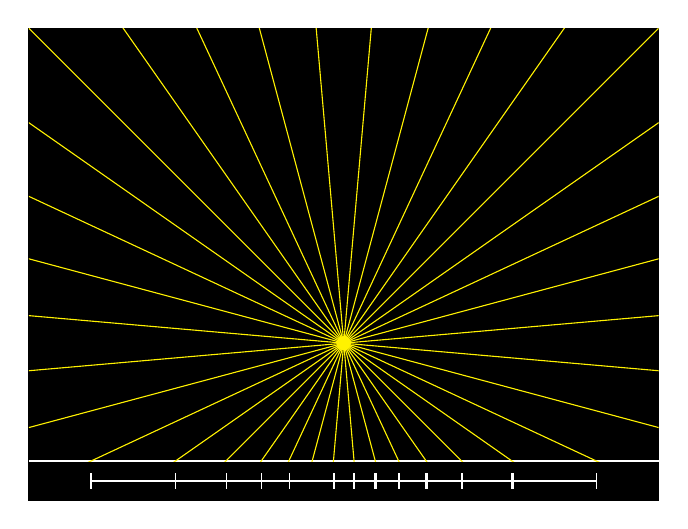
\begin{tikzpicture}
  \draw[fill=black,black] (-4,-2) rectangle (4,4);
  \draw[fill=yellow] (0,0) circle [radius=0.1cm];
  s\draw[thick,white,name path=wall] (-4,-1.5) -- (4,-1.5);

  \begin{scope}
    \path[clip] (-4,-1.5) rectangle (4,4);

    \foreach[count=\i] \x in {-95,-85,...,260} {
      \draw[thin,yellow,name path={ray}] (0,0) -- (\x:8);
      \path[name intersections={of=wall and ray,by=h\i}];
    }
  \end{scope}

  \foreach[count=\i] \j in {2,...,4,5,6,7,8,35,34,33,32,31} {
    \draw[white,|-|] ($ (h\i) + (0,-0.25) $) -- ($ (h\j) + (0,-0.25) $);
  }
\end{tikzpicture}

\end{document}